
\chapter{Konstrukce důkazu}

Představme hypotézu, kterou se snažíme ověřit.
\begin{hypot}\label{veta02:hypoteza}
Mějme přípustnou posloupnost $p=(p_k | 3 \leq k \neq 6)$ a neutrální posloupnost $q=(q_k \mid 3 \leq k \neq 6)$, pak existuje takové přirozené $n$, že $p+nq$ je přijatelná.
\end{hypot}


V článku \citep{Samal09} autoři naznačují konstrukci důkazu, za předpokladu, že existují nějaké pomocné grafy. V další kapitole představíme způsob, jak takové grafy hledat. Teď se zaměříme na důkaz samotný, respektive nejprve představíme graf, který v důkazu pomáhal již Eberhardovi.

\section{Triarky a operace s nimi}

\begin{definice}[Triark]\label{def02:1}
Triark je takový rovinný graf $T$, že vrcholy jeho vnější stěny tvoří cyklus $C$, každý vnitřní vrchol (tj. vrcholy $T-C$) má v $T$ stupeň právě 3 a v $C$ jsou tři navzájem různé vrcholy $x$, $y$, $z$ stupně 2 - \textbf{rohy}, že vrcholy každé ze tří cest v C, které vzniknou odstraněním rohů z C, mají střídavě stupeň 2 a 3, počínaje i konče stupněm 2.
\end{definice}

\textbf{Strana} triarku je každá z výše zmíněných cest v C, ke které na oba konce připojíme i příslušný roh. \textbf{Délka strany} triarku odpovídá počtu jejích vnitřních vrcholů stupně 2 v T. O triarku se stranami délky $a$, $b$, $c$ mluvíme jako o ($a$, $b$, $c$,)-\textbf{triarku}. Poznamenejme, že na pořadí stran v názvu nezáleží (odpovídají rotacím). Později využijeme ještě dalšího značení. $M$-\textbf{triark} má vnitřní strany pouze velikostí z $M$. U triarku přejímáme některé termíny používané pro trojúhelníky a jejich význam bude vždy intuitivní.

\begin{figure}[h!]\centering
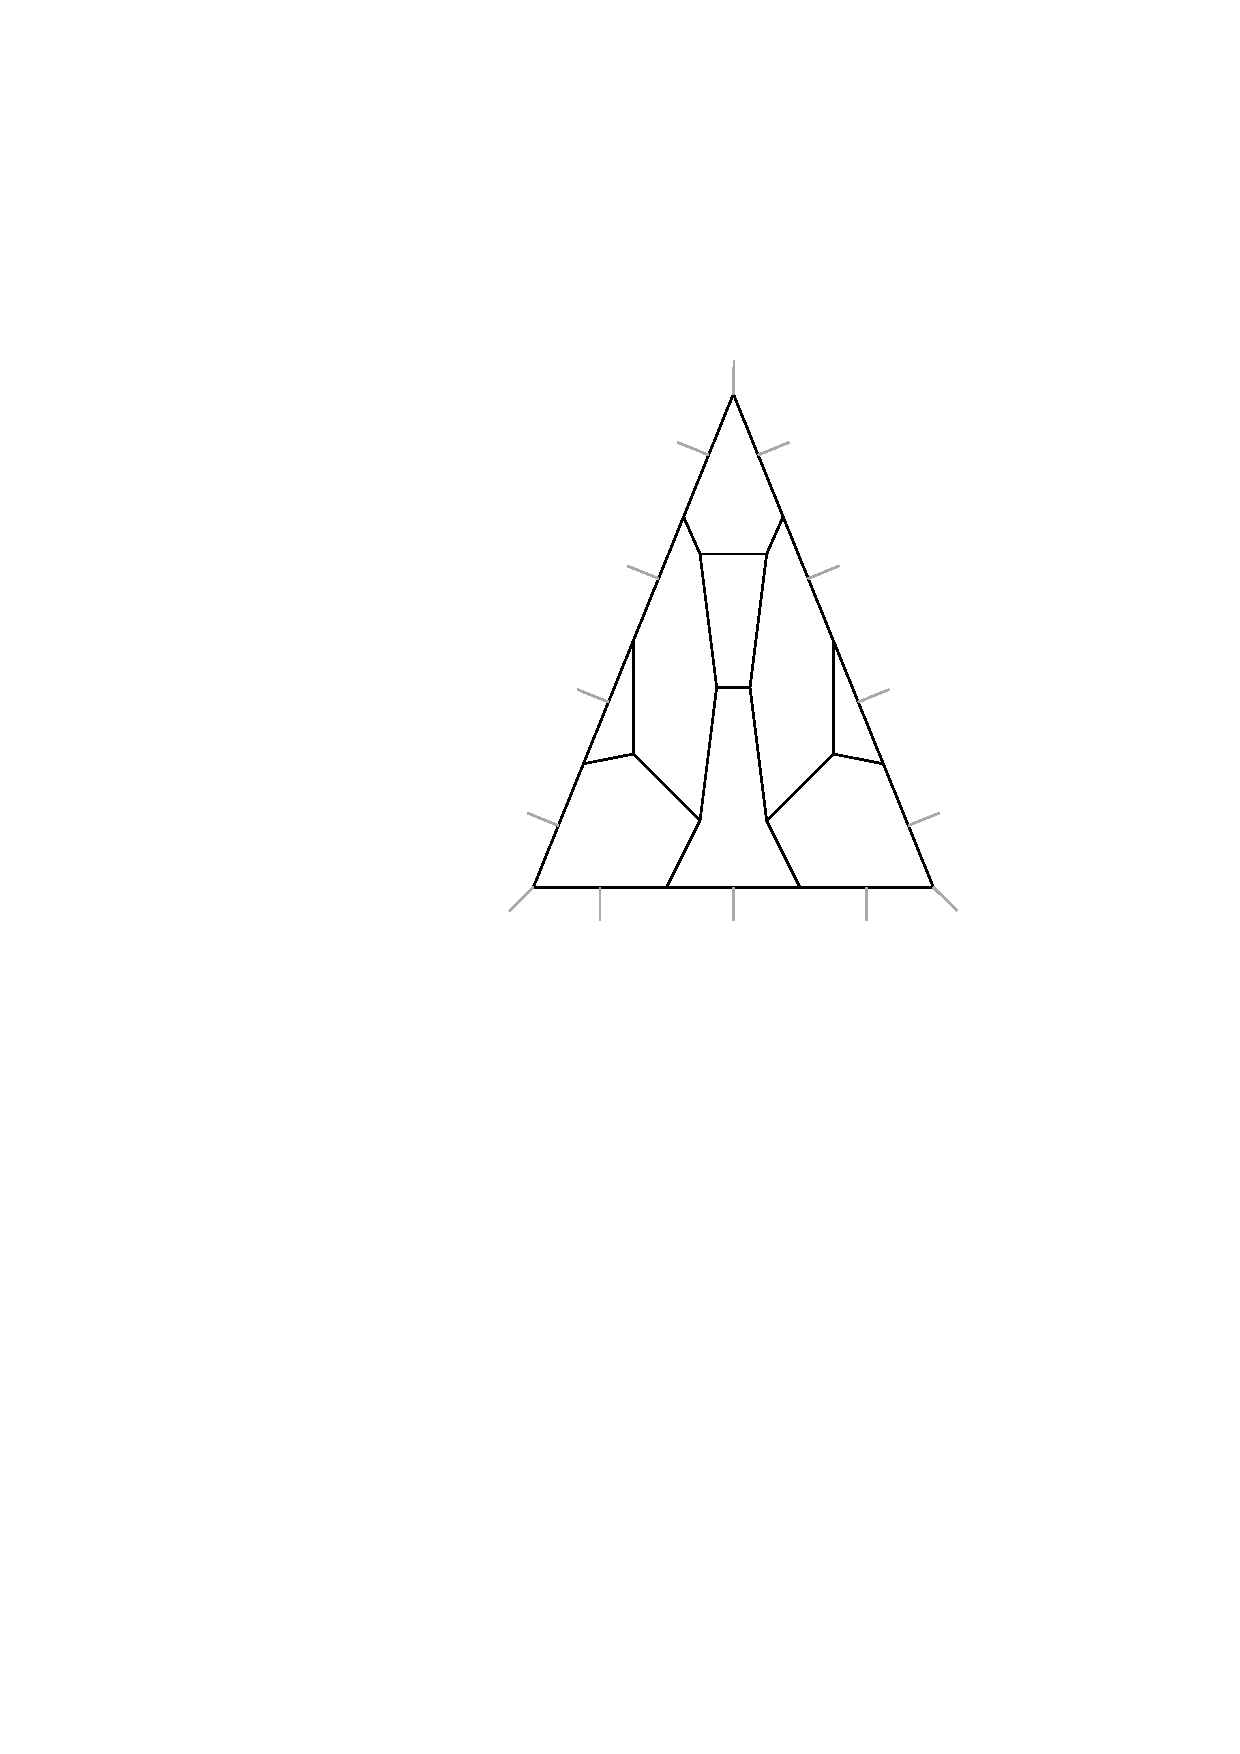
\includegraphics[height=60mm]{../img/triarc}
\caption{Ukázka (4,4,3)$ \lbrace 4,7\rbrace $-triarku.}
\label{obr03:triark}
\end{figure}

Zmiňme velmi užitečnou vlastnost triarků: pokud máme dva triarky, oba mající stranu stejné délky, můžeme je za tuto stranu slepit a získáme opět graf, jehož vnitřní vrcholy mají stupeň 3. (Při slepovaní se ztotožní vždy vrchol stupně 2 s vrcholem stupně 3.) Pokud slepíme triarky tak, že protější strany výsledného grafu budou stejně dlouhé (tedy speciálně při slepení dvou stejný triarků), budeme podle jeho tvaru mluvit o \textbf{rovnoběžníku}. Rovnoběžníky jdou navíc slepovat podobně jako triarky a můžeme tím každý již existující rovnoběžník zvětšit na libovolný rozměr, který je násobkem jeho původních rozměrů.


\begin{figure}[h!]\centering
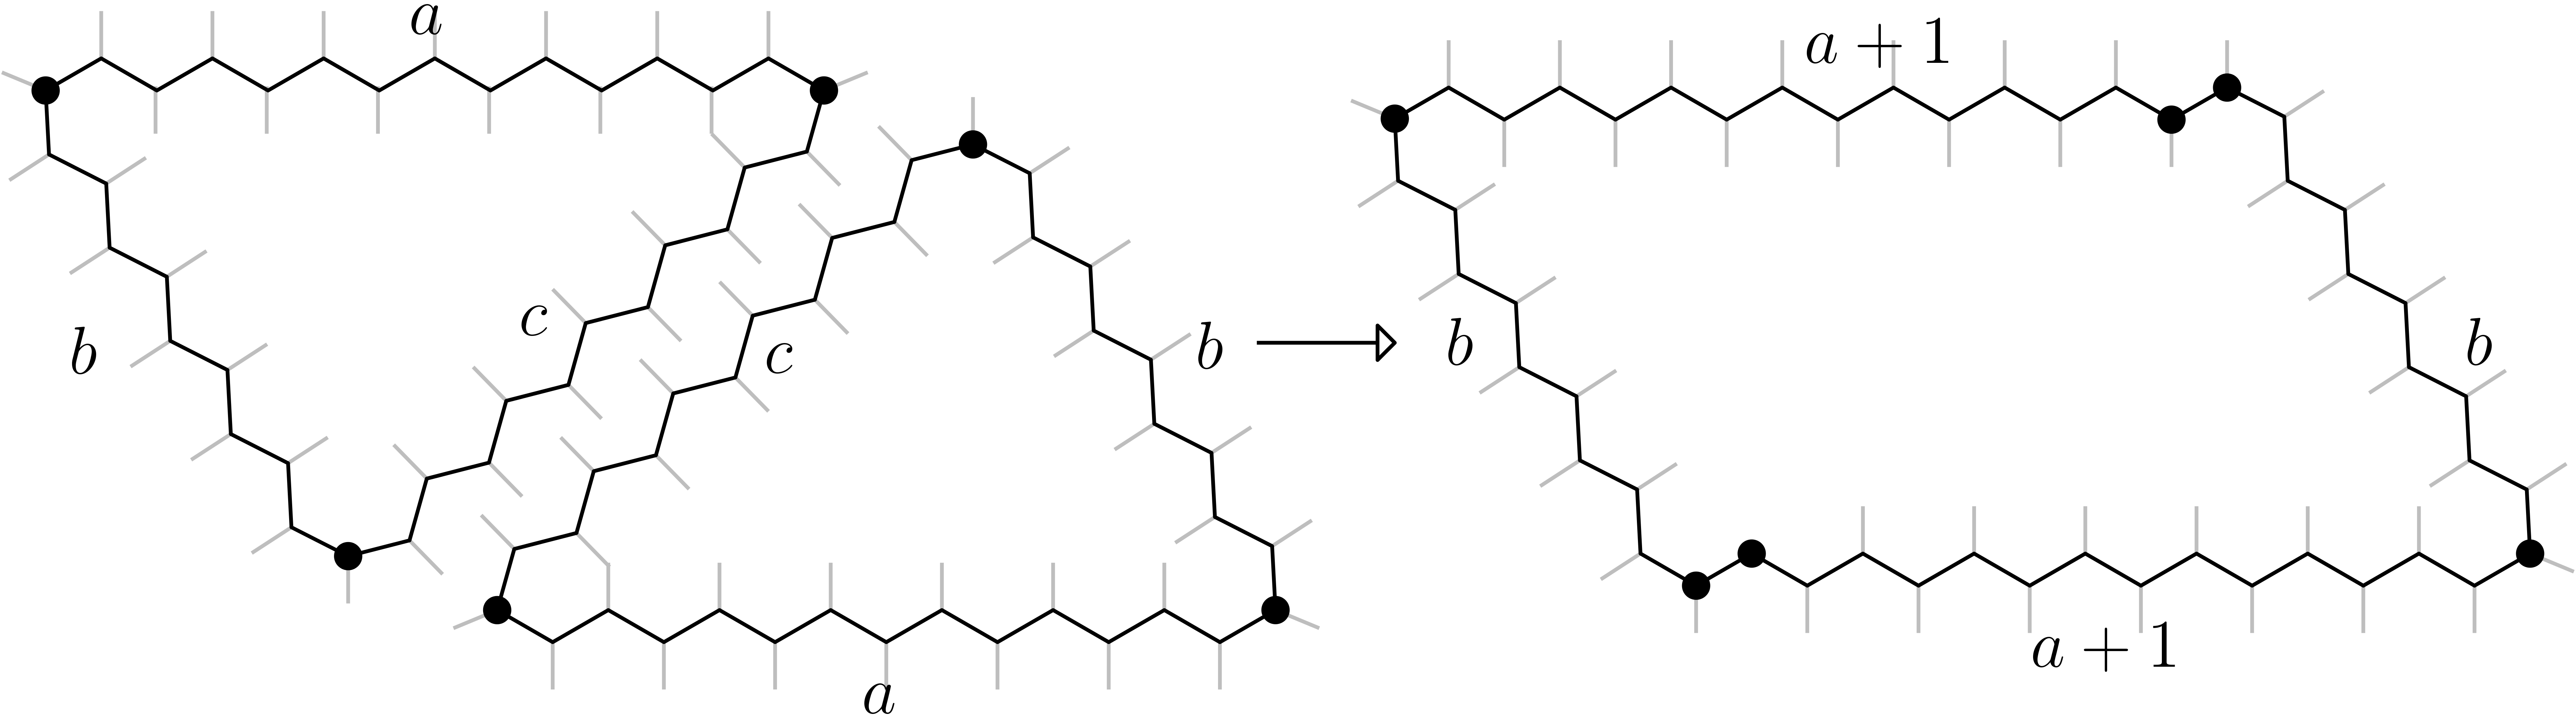
\includegraphics[width=\textwidth]{../img/T-P}
\caption{Spojení dvou triarků za vzniku rovnoběžníku.}
\label{obr21:T-P}
\end{figure}

Mohli bychom ale chtít spojovat triarky tak, aby výsledkem byl opět triark. Mějme ($a_1$, $b_1$, $c_1$)-triark a ($a_2$, $b_2$, $c_2$)-triark a vhodný rovnoběžník. Slepením, jako na obrázku \ref{obr22:T-T}, vznikne ($a_1+a_2$, $b_1+b_2$, $c_1+c_2$)-triark. 

\begin{figure}[h!]\centering
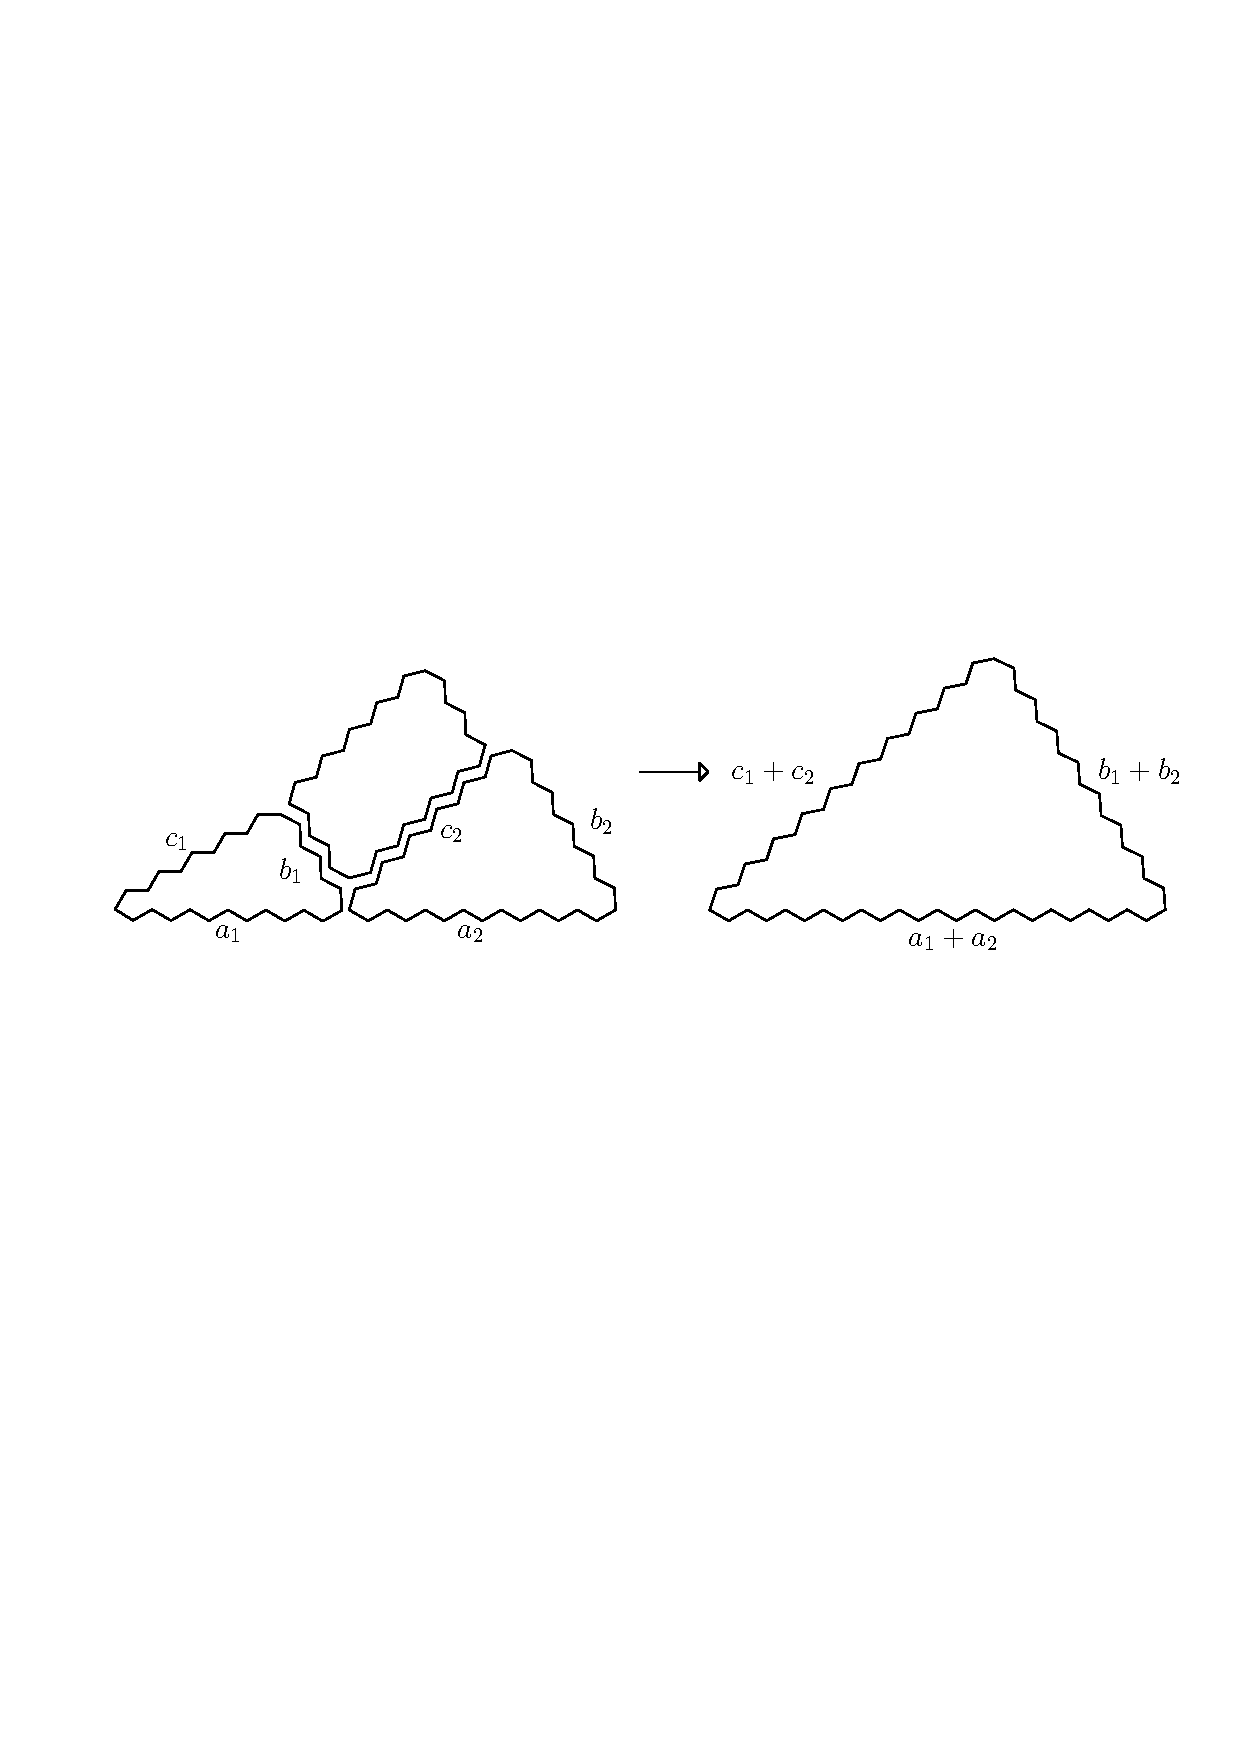
\includegraphics[width=\textwidth]{../img/T-T}
\caption{Spojení triarků spolu s rovnoběžníkem za vzniku triarku.}
\label{obr22:T-T}
\end{figure}

A závěrem budeme chtít spojit dva triarky tak, aby výsledkem byl kubický graf (tedy aby nevznikly žádné nové stěny s vrcholy stupně dva). Graf, který má tuto funkci označíme za \textbf{prstenec}. Pro lepší představu si prstenec představujme jako plášť trojbokého hranolu, triarky jako dolní a boční podstavu. Na všech podstavných hranách dojde ke splynutí vrcholů triarků s vrcholy prstence a vznikne graf nakreslitelný na hranol (tedy tedy i na sféru), takže výsledkem je rovinný graf. Zadefinujme prstenec. Prstenec je souvislý graf, ve kterém můžeme vyznačit dva disjunktní cykly tak, že stupně vrcholů každého cyklu jsou opačné než stupně příslušných triarků, které chceme spojit. Kde opačně znamená záměna dvoj- a tří- vaznosti vrcholů. Pro případné dokreslení můžeme použít obrázek \ref{obr03:konstrukceiv}, na kterém je speciální druh prstence. 

%\begin{figure}[h!]\centering
%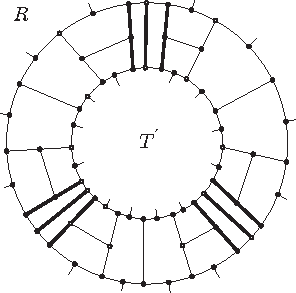
\includegraphics[height=40mm]{../img/T-G}
%\caption{Spojení triarků prstencem za vzniku kubického grafu.}
%\label{obr23:T-G}
%\end{figure}


\section{Důkaz za předpokladu existence pomocných grafů}
Převeďme hypotézu ve větu.

\begin{veta}\label{veta02:2}
Mějme přípustnou posloupnost $p=(p_k | 3 \leq k \neq 6)$ a neutrální posloupnost $q=(q_k \mid 3 \leq k \neq 6)$ a následující grafy pro nějaké přirozené k:
\begin{description}
\item[(i)] ($k$, $k$, $k$),$Q$-triark;
\item[(ii)] ($k$, $k$, $k-1$),$Q$-triark;
\item[(iii)] rovnoramenný $Q\cup \lbrace1\rbrace$-triark, délky jehož stejných stran jsou dělitelné $k$ a který obsahuje právě jednu stěnu velikosti $l$ pro každé nenulové $p_l$ v $p$, této stěně říkejme \textbf{jádro} triarku;
\item[(iv)] prstenec, který dokáže spojit dva stejně velké, rovnostranné triarky.
\end{description}

Pak existuje takové přirozené $n$, že $p+nq$ je přijatelná.
\end{veta}


Myšlenka důkazu pak není příliš složitá: každou stěnu ze zadané posloupnosti $p$ zabalíme do triarku (iii), připravíme si pomocné lepící a zkrášlující prvky (ii), díky kterým získáme jediný velký rovnostranný triark. K němu zkonstruujeme ještě jeden se stejně dlouhými (i) a pomocným prstencem je spojíme v kýžený graf (iv). Všechny tyto pomocné objekty jsou totiž (kromě jader) jen ze stěn, které jsou v zadané neutrální posloupnosti, lepicí operace zachovávají kubičnost uvnitř grafu a prstenec pak spojí dva triarky v hledaný kubický graf.

\textit{Důkaz.} Nejprve slepíme dva ($k$, $k$, $k-1$)-triarky za stěnu délky $k$ a získáme rovnoběžník se všemi stranami délky $k$. A díky slepování můžeme získat i libovolný rovnoběžník o rozměrech $mk$, $lk$ pro $m$, $l$ přirozená. Poté postupně spojujeme jednotlivé jádrové triarky za pomoci příslušného lichoběžníku, dokud nezískáme jediný triark, který obsahuje všechny stěny z $P$.

Zkusme vzniklý triark upravit na rovnostranný. Při slepování triarků se velikosti výsledných stran rovnají součtům původním. Pokud tedy slepujeme s ($k$, $k$, $k-1$)-triarkem, zmenšíme vždy tu stěnu, na kterou připadne rozměr $k-1$, vůči ostatním. Takže pokud budeme opakovat lepení výsledného triarku, v každém kroku se součet rozdílů mezi stranami zmenší a tedy nutně získáme rovnostranný triark. Modifikujme ho stejnou operací, aby zůstal rovnostranný, ale navíc délka jeho stran byla násobkem $k$ a označme výsledný triark $T_1$.

Slepováním ($k$,$k$,$k$)-triarků z (i) spolu s $k$,$k$ rovnoběžníky získáme druhý triark $T_2$ o stejném rozměru jako $T_1$. Kdybychom celý problém řešili na tóru, stačilo by $T_1$ a $T_2$ spojit do rovnoběžníku a sjednotit odpovídající strany. Na kouli místo toho použijeme prstenec z (iv). Tím získáme graf, který je kubický, rovinný a obsahuje požadované stěny. $\square$

Všimněme si, že větu jde jednoduše zesílit: nejen že za splnění předpokladů existuje nějaké $n \in \mathbb{N}$, pro které je $p+nq$ přijatelná; existuje jich libovolně mnoho. V důkazu stačí před spojením $T_1$ a $T_2$ prstencem nejprve oba triarky slepit s dalšími instancemi $T_2$ tak, aby vznikly nové, stejně velké rovnostranné triarky $T_{1}^*$ a $T_{2}^*$. Tímto způsobem lze libovolně zvětšit $n$. $T_{1}^*$ a $T_{2}^*$ pak opět spojíme prstencem.